\documentclass{report}

\input{~/dev/latex/template/preamble.tex}
\input{~/dev/latex/template/macros.tex}
\graphicspath{{./}}

\title{\Huge{2.1 HW Solutions}}
\author{\huge{Nathan Warner}}
\date{\huge{Jan 17, 2023}}

\begin{document}
    \maketitle
    \section{\Large{Question 1}}

    \bigbreak \noindent 
    \qs{}{A tank holds 3,000 gallons of water, which drains from the bottom of the tank in half an hour. The values in the table show the volume V of water remaining in the tank (in gallons) after t minutes.}
    
    \bigbreak \noindent 
    \textbf{A).} If P is the point (15, 765) on the graph of V, find the slopes 
    of the secant lines PQ when Q is the point on the graph with t = 5, 10, 20, 25, and 30. 
    (Round your answers to one decimal place.)
    
    \pf{Solution:}{
    }
    \textbf{1. (5,2070)} 

    \begin{align*}
        \frac{2070-765}{5-15} =-130.5
    .\end{align*}

    \textbf{2. (10,1329)}
    
    \begin{align*}
        \frac{1329-765}{10-15} = -112.8     
    .\end{align*}

    \textbf{3. (20,348)}

    \begin{align*}
        \frac{348-765}{20-15} = -83.4
    .\end{align*}

    \textbf{4. (25,81)}
    
    \begin{align*}
        \frac{81-765}{25-15} = -68.4
    .\end{align*}

    \textbf{5. (30,0)}
    
    \begin{align*}
        \frac{0-765}{30-15} = -51
    .\end{align*}

    \bigbreak \noindent 
    \textbf{B).} Estimate the slope of the tangent line at P by averaging the slopes of the two adjacent secant lines corresponding to the two points closest to P. (Round your answer to one decimal place.)
    
    \pf{solution:}{}
    The two points closest to P are (10,1329) and (20,348), we take the average of both 
    their slopes and get \textbf{-98.1}
    
    \pagebreak
    \section{\Large{Question 2}}

    \bigbreak \noindent \bigbreak \noindent 
    \qs{}{The point P(6,-4) lies on the curve, $y= \frac{4}{5-x}$}

    \bigbreak \noindent 
    \textbf{A).} if Q is the point $ \left(x, \frac{4}{5-x}\right) $ 
    find the slope of the secant line PQ (correct to six decimal places) 
    for the following values of x.

    \bigbreak \noindent 
    \textbf{i.)} x = 5.9

    \begin{large}
        \begin{align*}
            \frac{-4- \frac{4}{5-5.9}}{6-5.9}
            =4.\overline{4}
        .\end{align*}
    \end{large}
    
    \bigbreak \noindent 
    \textbf{B).} Using the results of part (a), guess the value of the slope of the tangent 
    line to the curve at P(6,-4) 
    
    \bigbreak \noindent 
    \pf{Solution:}{}
        The numbers appear to be get closer and closer to 4, so the slope of the tangent line
        at P(6,-4) is likely 4

    \bigbreak \noindent \bigbreak \noindent 
    \textbf{C).} Using the slope from part (b), find an equation of the tangent line 
    to the curve at P(6,-4)

    \bigbreak \noindent 
    \pf{Solution:}{}
    \textbf{If} the equation for a line is
    \begin{align*}
        y-y_1=m \left(x-x_1'\right)
    .\end{align*}
    \textbf{And} the slope of the tangent line is 4, then the equation would be,
    \begin{center}
        $y- \left(-4\right) = 4 \left(x-6\right)$ \\
        y + 4 = $4x-24$ \\ 
        $y=4x-28$
    \end{center}
    
    \pagebreak
    \section{\Large{Question 3}}
        \qs{}{If a rock is thrown upward on the planet Mars with a velocity 18 m/s, 
       its height in meters t seconds later is given by $y = 18t - 1.86t^2.$ 
       (Round your answers to two decimal places.) 
    }

    \bigbreak \noindent 
    \textbf{A).} Find the average velocity in m/s over the given time interval  
   
    \bigbreak \noindent 
    \textbf{(i) [1,2]} 
    \begin{align*}
        y \left(1\right) = 18 \left(1\right) - 1.86 \left(1\right) ^2 \\
        y \left(1\right) = 16.14
    .\end{align*}

    \bigbreak \noindent  
    \begin{align*}
        y \left(2\right) = 18 \left(2\right) - 1.86 \left(2\right) ^2 \\ 
        y \left(2\right) = 28.56 
    .\end{align*}

    \bigbreak \noindent 
    \textbf{So} we have the points (1,16.14) and (2,28.56) so we can plug into average 
    velocity equation

    \bigbreak \noindent 
    \begin{align*}
        Average\ velocity = \frac{28.56 - 16.14}{2-1} \\
        = 12.42 m \diagdown s
    .\end{align*}

    \pagebreak
    \section{\Large{Question 4}}

    \bigbreak \noindent \bigbreak \noindent 
    \qs{}{The table shows the position of a motorcyclist after accelerating from rest.}
    
    \bigbreak \noindent 
    \begin{center}
        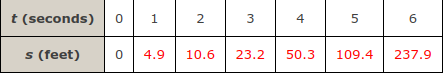
\includegraphics[scale=0.7]{hw4.png}
    \end{center}
    
    \bigbreak \noindent 
    \textbf{(a) Find the average velocity (in ft/s) for each time period.}
    
    \bigbreak \noindent 
    \textbf{(i) [2,4]}
    
    \bigbreak \noindent 
    \textbf{So}, we use the average velocity formula with values at t = 2 and t = 4
    
    \begin{align*}
        Average\ velocity = \frac{50.3-10.6}{4-2} \\
        = 19.85 
    .\end{align*}

    \bigbreak \noindent 
    \textbf{(b)} Plot the points in the table to create a graph of s as a function of t to estimate the instantaneous velocity (in ft/s) when t = 3. (Round your answer to one decimal place.)
    
    \bigbreak \noindent 
    \pf{solution:}{}
    
\end{document}

